\chapter{Specifikace cílů práce}

%% \section{Zadání}
%% % ZADANI (bude vlozeno jako prvni stranka diplomove prace):
%% %
%% % Seznamte se se základními principy používanými při objektově
%% % orientovaném návrhu a implementaci, konkrétně s low coupling, high
%% % cohesion a Law of Demeter. Popište pravidla, která umožní ověřování
%% % těchto principů. Vytvořte nástroj, který umožní analyzovat kód v
%% % jazyce Java a vyhodnocovat vámi definovaná pravidla. Činnost
%% % nástroje ověřte na vzorových příkladech kódu. Při návrhu nástroje se
%% % zaměřte na jeho budoucí rozšiřitelnost.

\section{Cíle práce}
\begin{itemize}
\item definovat jazyk pro zadávání pravidel
\item specifikovat pravidla pro návrhové principy \emph{Law of Demeter}, \emph{low coupling} a \emph{high cohesion}
\item vytvořit nástroj, který umožní ověřovat pravidla v reálném projektu
\end{itemize}

\section{Struktura výsledného systému}
Globální sturktura výsledné práce je na obrázku \ref{global_structure}.

\begin{figure}[h!]
  \centering
  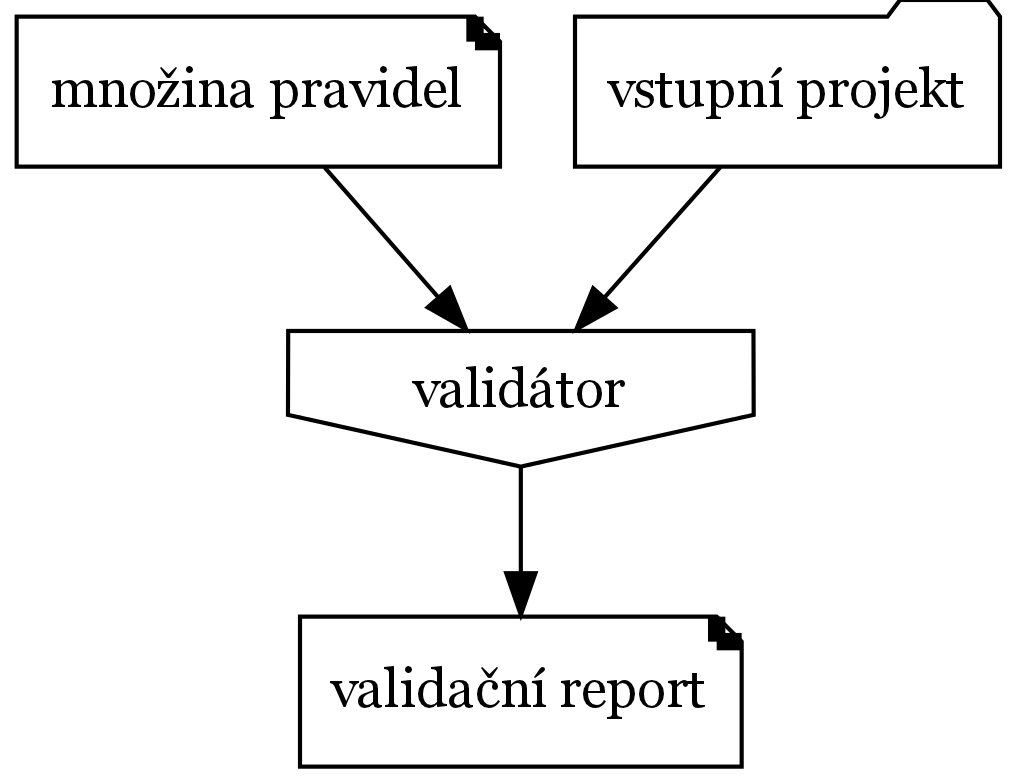
\includegraphics[width=0.5\textwidth]{./graphs/global_structure.png}
  \caption{Znázornění hlavních součástí práce.\label{global_structure}}
\end{figure}

\section{Funkční požadavky na výsledný systém}

\section{Nefunkční požadavky na výsledný systém}
\begin{itemize}
\item TODO: (NetBeans platform) -> není v zadaní specifikováno (spíš navrhnout v části Návrh)
\item systém bude fungovat nad instancemi programovacího jazyka Java 6 (projekty napsané v jazyku Java)
\item systém bude umožňovat definovat další pravidla
\end{itemize}

\section{Rešerše existujících řešení}
\label{requirements-existing_tools}
% TODO: do background research on positives and negatives of these tools
% TODO: v rychlosti zopakovat rešerši na nové nástroje a konkrétní vlastnosti, které jsou důležité pro tuto práci

\subsection{JDepend}

\begin{itemize}
\item \href{http://www.clarkware.com/software/JDepend.html}{http://www.clarkware.com/software/JDepend.html}
\item nástroj pro testování kvality návrhu
\item pracuje nad \verb+*.class+ soubory (získává data z bytekódu)
\end{itemize}

\subsection{QJ-Pro}
\begin{itemize}
\item \href{http://qjpro.sourceforge.net}{http://qjpro.sourceforge.net}
\end{itemize}

\subsection{DP-Miner}
\begin{itemize}
\item \href{http://www.utdallas.edu/~yxz045100/DesignPattern/DP\_Miner/}{http://www.utdallas.edu/~yxz045100/DesignPattern/DP\_Miner/}
\item hledání návrhových vzorů v existujících projektech
\item článek: Jing Dong and Yajing Zhao, Experiments on Design Pattern Discovery \\ (\href{http://www.utdallas.edu/~jdong/papers/PROMISE07.pdf}{http://www.utdallas.edu/~jdong/papers/PROMISE07.pdf})
\end{itemize}

\subsection{Macker}
\begin{itemize}
\item \href{http://innig.net/macker/}{http://innig.net/macker/}
\item build-time architectural rule checking utility for Java developers
\item zpracovává \verb+*.class+ soubory (bytekód)
\end{itemize}

TODO: přidat

\begin{itemize}
\item CheckStyle -- \href{http://checkstyle.sourceforge.net/}{http://checkstyle.sourceforge.net/}
\item PMD -- \href{http://pmd.sourceforge.net/}{http://pmd.sourceforge.net/}
\end{itemize}



\begin{itemize}
\item Popis řešeného problému, vymezení cílů DP/BP a požadavků na implementovaný systém.

\item Rešeršní zpracování existujících implementací, pokud jsou známy.
  %% zde budou výsledky rešerše souvisejících nástrojů

\end{itemize}
